\documentclass[12pt]{article}

\usepackage[margin=1in]{geometry}
\usepackage{amsmath, amssymb, amsthm, amsfonts}
\usepackage{tikz}
\usepackage{hyperref}
\usepackage{url}

% ------------------------------------------------------------
% Theorem Environments
% ------------------------------------------------------------
\theoremstyle{plain}
\newtheorem{theorem}{Theorem}[section]
\newtheorem{lemma}[theorem]{Lemma}
\newtheorem{proposition}[theorem]{Proposition}
\newtheorem{corollary}[theorem]{Corollary}

\theoremstyle{definition}
\newtheorem{definition}[theorem]{Definition}
\newtheorem{example}[theorem]{Example}
\newtheorem{remark}[theorem]{Remark}

% ------------------------------------------------------------
% Title and Author
% ------------------------------------------------------------
\title{\textbf{Unification of Linguistics Through a Generalized Theory of\\
the Universal Linguistic Functor (ULF)}}
\author{
  \textbf{Matthew Long}\\
  \textit{Magneton Labs}
}
\date{\today}

\begin{document}
\maketitle

\begin{abstract}
We present a generalized theory of the Universal Linguistic Functor (ULF) that aims to unify core principles of syntax, semantics, and cross-linguistic variation under a category-theoretic framework. We develop the concept of a universal grammar object as an initial object in the category of grammars, extend this to presheaves capturing language-specific parameters, and show how enriched category structures and topos theory can yield a graded and context-sensitive semantics. We provide detailed mathematical formulations and proof sketches for key propositions and theorems, illustrating the formal foundations of ULF. Finally, we discuss potential applications to natural language processing (NLP) and cognitive modeling, underscoring the practical value of a unifying category-theoretic approach.
\end{abstract}

\tableofcontents

\section{Introduction}\label{sec:intro}
A central goal in linguistics is to find a unifying perspective that can explain both the universality and the variability of human languages. The \emph{Universal Linguistic Functor (ULF)} framework seeks to realize this goal by applying the tools of category theory, which has already proved successful in unifying various areas of mathematics and theoretical computer science.

The key ambitions of the ULF framework include:
\begin{enumerate}
    \item Treating \emph{universal grammar} as an \textbf{initial object} in the category of grammars \(\mathbf{Gram}\).
    \item Capturing \textbf{cross-linguistic variation} via \textbf{presheaves} over a category of linguistic contexts.
    \item Introducing \textbf{enriched} and \textbf{topos-theoretic} semantics to handle gradience, context, and intensional phenomena.
\end{enumerate}

This paper expands on an earlier formulation of ULF, providing additional mathematical details and more comprehensive proof sketches. We explain how standard techniques from category theory---functors, adjunctions, presheaves, monads, and toposes---coalesce into a powerful framework for modeling language in a structurally consistent way. The synergy between ULF and computational models in NLP further highlights the practical promise of this approach.

\section{Background and Motivation}

\subsection{Category Theory as a Unifying Language}
Category theory is often described as the mathematics of structure and composition. Its abstract perspective has proven fruitful in a wide range of fields, from algebraic geometry and homotopy theory to theoretical computer science, type theory, and even physics.

\begin{definition}[Category]
A \emph{category} \(\mathbf{C}\) consists of:
\begin{itemize}
    \item a class of \emph{objects},
    \item a class of \emph{morphisms} (also called arrows) between these objects,
\end{itemize}
such that morphisms compose associatively and there is an identity morphism for every object.
\end{definition}

Linguistics can be cast in these terms by regarding grammatical constructs as objects and derivational or interpretive processes as morphisms. By building on these abstractions, we can flexibly model the interplay between syntax, semantics, and cross-linguistic constraints.

\subsection{Functors, Natural Transformations, and Adjointness}
\begin{definition}[Functor]
Given categories \(\mathbf{C}\) and \(\mathbf{D}\), a \emph{functor} \(F: \mathbf{C} \to \mathbf{D}\) assigns to each object \(C \in \mathbf{C}\) an object \(F(C) \in \mathbf{D}\) and to each morphism \(f: C \to C'\) a morphism \(F(f): F(C) \to F(C')\), preserving identities and composition.
\end{definition}

In linguistics, functors can encode the mapping from syntactic derivations to semantic interpretations. A \emph{natural transformation} between functors represents a systematic way of transforming one functor into another while respecting the underlying category structures. Adjoint functors capture fundamental correspondences (e.g., the syntax-semantics interface in certain formulations \cite{BarkerShan}).

\subsection{Topos Theory and Set-Theoretic Generalizations}
A \emph{topos} is often described as a generalization of set theory. A Grothendieck topos is a category that behaves sufficiently like \(\mathbf{Set}\), equipped with a subobject classifier and an internal logic. Topos theory can treat intensional or context-dependent phenomena, making it a robust candidate for modeling aspects of language that transcend simple truth-conditional semantics.

\section{The Category of Grammars \(\mathbf{Gram}\)}
We formally define the category \(\mathbf{Gram}\), whose objects are grammars and whose morphisms are grammar homomorphisms.

\subsection{Objects: Formal Grammars}
\begin{definition}[Formal Grammar]
A \emph{formal grammar} \(G\) is specified by:
\[
G = (N, \Sigma, P, S),
\]
where \(N\) is a set of nonterminal symbols, \(\Sigma\) is a set of terminal symbols, \(P\) is a set of production rules or constraints, and \(S \in N\) is a distinguished start symbol. More generative frameworks (e.g., Minimalist Grammars, TAGs, HPSG) can also be encoded as objects in \(\mathbf{Gram}\) by abstracting their structural relations.
\end{definition}

\subsection{Morphisms: Grammar Homomorphisms}
\begin{definition}[Grammar Homomorphism]
\label{def:grammar-homomorphism}
Let \(G_1 = (N_1, \Sigma_1, P_1, S_1)\) and \(G_2 = (N_2, \Sigma_2, P_2, S_2)\) be two grammars. A \emph{grammar homomorphism} \(\phi: G_1 \to G_2\) consists of:
\begin{itemize}
    \item A function \(\phi_N: N_1 \to N_2\) that preserves start symbols (\(\phi_N(S_1) = S_2\) or an equivalent designated object in \(G_2\)).
    \item A function \(\phi_\Sigma: \Sigma_1 \to \Sigma_2\) that respects terminal correspondences (often identity or subset mappings).
    \item A mapping of production rules \(p \in P_1\) to rules in \(P_2\) that is consistent with the images of \(N_1\) and \(\Sigma_1\).
\end{itemize}
\end{definition}

\begin{definition}[The Category \(\mathbf{Gram}\)]
\(\mathbf{Gram}\) is the category whose objects are formal grammars and whose morphisms are grammar homomorphisms as defined in Definition \ref{def:grammar-homomorphism}. Composition is given by composing the component functions \(\phi_N\) and \(\phi_\Sigma\) and verifying that production rules map consistently. Identities are the obvious identity mappings.
\end{definition}

\section{Universal Grammar as an Initial Object}
A cornerstone of the ULF framework is the hypothesis that there exists a \emph{universal grammar object}, representing the minimal universal feature set and constraints that can generate every possible human grammar through systematic parameterization or specialization.

\subsection{Definition and Statement of Existence}
\begin{definition}[Initial Object]
An object \(I\) in a category \(\mathbf{C}\) is \emph{initial} if for every object \(C\) in \(\mathbf{C}\), there exists a unique morphism \(I \to C\).
\end{definition}

\begin{theorem}[Universal Grammar Object]\label{thm:UG}
Assume there is a set of universal principles/features such that every grammar \(G\) arises from fixing these principles in specific ways. Then there exists an \emph{initial object} \(\mathcal{U} \in \mathbf{Gram}\), called the \emph{universal grammar object}, satisfying:
\[
\forall G \in \mathbf{Gram}, \quad \exists! \; (\mathcal{U} \to G).
\]
\end{theorem}

\begin{proof}[Sketch]
Construct a ``free grammar'' on the universal feature set. This involves:
\begin{enumerate}
    \item \textbf{Define the Generators:} Let \(\mathcal{F}\) be the set of minimal syntactic categories, universal constraints (e.g., bounding nodes for movement), morphological principles, etc.
    \item \textbf{Introduce Relations:} Suppose \(\mathcal{R}\) is the set of universal constraints (e.g., locality constraints, case assignment). We consider the quotient of the free grammar on \(\mathcal{F}\) by closure under \(\mathcal{R}\).
    \item \textbf{Universal Property:} Every grammar \(G\) is a quotient under a homomorphism that interprets each universal generator in \(G\). Uniqueness follows from the fact that once these generator images are fixed, the entire grammar is determined.
\end{enumerate}
This construction fulfills the criteria for an initial object in \(\mathbf{Gram}\).
\end{proof}

\section{Presheaf-Based Language Variation}

\subsection{Category of Linguistic Contexts \(\mathbf{Lin}\)}
To capture systematic \emph{variation} across languages, we introduce the category \(\mathbf{Lin}\) whose objects are parameter configurations (e.g., morphological constraints, word-order types), and whose morphisms represent parameter adjustments or refinements.

\subsection{Presheaves for Capturing Variation}
\begin{definition}[Presheaf]
Given a category \(\mathbf{C}\), a \emph{presheaf} on \(\mathbf{C}\) is a functor \(P: \mathbf{C}^{op} \to \mathbf{Set}\).
\end{definition}

In our setting,
\[
P: \mathbf{Lin}^{op} \to \mathbf{Set},
\]
assigns to each linguistic context \(L\) the set \(P(L)\) of possible derivations or grammatical realizations consistent with \(L\). Restriction maps handle how these sets change when one moves along morphisms in \(\mathbf{Lin}\).

\subsection{Commutative Diagrams and Natural Transformations}
Let \(P, Q: \mathbf{Lin}^{op} \to \mathbf{Set}\) be two presheaves capturing different modules (e.g., syntax and morphology). A \emph{natural transformation} \(\alpha: P \to Q\) imposes consistency across modules.

\begin{theorem}[Presheaf Consistency]\label{thm:PresheafConsistency}
If \(\alpha: P \to Q\) is a natural transformation, then for any morphism \(\sigma: L_2 \to L_1\) in \(\mathbf{Lin}\), the following diagram commutes:
\[
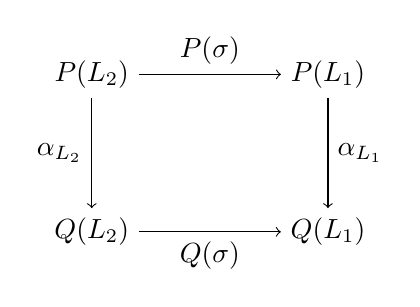
\begin{tikzpicture}[node distance=4em, auto]
  \node (P2) at (0,0) {$P(L_2)$};
  \node (P1) at (3,0) {$P(L_1)$};
  \node (Q2) at (0,-2) {$Q(L_2)$};
  \node (Q1) at (3,-2) {$Q(L_1)$};

  \draw[->] (P2) to node {$P(\sigma)$} (P1);
  \draw[->] (Q2) to node [below] {$Q(\sigma)$} (Q1);
  \draw[->] (P2) to node [left] {$\alpha_{L_2}$} (Q2);
  \draw[->] (P1) to node [right] {$\alpha_{L_1}$} (Q1);
\end{tikzpicture}
\]
Hence, parameter changes in \(\mathbf{Lin}\) yield consistent transformations in the syntactic and morphological modules.
\end{theorem}

\begin{proof}[Sketch]
By the definition of a natural transformation, for each object \(L\in \mathbf{Lin}\) we have a function \(\alpha_L: P(L) \to Q(L)\). The naturality condition requires square commutativity for each morphism \(\sigma\). Hence, no contradiction arises when switching modules along parameter changes.
\end{proof}

\section{Enriched and Topos-Theoretic Semantics}

\subsection{Enrichment Over \texorpdfstring{$[0,1]$}{[0,1]} for Gradience}
Classical semantics often treats truth values as strictly Boolean. However, actual language usage reveals gradable adjectives and partial truth. We capture this with an \emph{enriched category} over \([0,1]\).

\begin{definition}[Enriched Category Over \texorpdfstring{$[0,1]$}{[0,1]}]
A category \(\mathbf{Sem}\) is \emph{enriched over} \(\bigl([0,1], \times, 1\bigr)\) if for each pair of objects \(A, B\), the morphisms \(\mathbf{Sem}(A,B)\) form an object in \([0,1]\). Composition is defined via the monoidal operation, typically multiplication.
\end{definition}

In linguistic terms, a morphism \(f: A \to B\) can represent a graded entailment or degree of membership. This approach aligns well with prototype theory in cognitive semantics.

\subsection{Topos-Theoretic Perspective}
A \emph{Grothendieck topos} \(\mathbf{E}\) can serve as a more general environment for intensional or context-sensitive semantics. If \(\mathbf{Lin}\) is regarded as a site with an appropriate Grothendieck topology, one can study:
\[
\mathrm{Sh}(\mathbf{Lin}), \quad\text{or}\quad \mathrm{PSh}(\mathbf{Lin}).
\]
The resulting internal logic in \(\mathbf{E}\) naturally encodes subobject classifiers, modal operators, and dynamic updates, offering a comprehensive semantic framework that accommodates intensional phenomena (e.g., belief contexts, possible worlds).

\section{Detailed Mathematical Formulations}

\subsection{Universal Grammar in the Monoidal Category of Small Categories}
We can view \(\mathbf{Gram}\) as an object in the monoidal category \(\mathbf{Cat}\) (the category of small categories) under \(\times\). Advanced formulations might explore:
\[
(\mathbf{Gram} \times \mathbf{Lin}), \quad (\mathbf{Gram} \times \mathbf{Sem}),
\]
or more intricate monoidal structures \(\otimes\). This perspective sets the stage for analyzing how grammar categories combine or factor through universal grammar objects.

\subsection{Monad Structures for Ambiguity}
Monads are pervasive in category theory and capture computational effects. In ULF, a monad can encode linguistic ambiguity or scopal variation:

\begin{definition}[Monad on \(\mathbf{Gram}\)]
A \emph{monad} on \(\mathbf{Gram}\) is an endofunctor \(T : \mathbf{Gram} \to \mathbf{Gram}\) equipped with unit \(\eta\) and multiplication \(\mu\) (both natural transformations) satisfying the standard monad axioms:
\[
\mu \circ T(\mu) = \mu \circ (\mu)_T, 
\quad
\mu \circ T(\eta) = \mathrm{id},
\quad
\mu \circ \eta_T = \mathrm{id}.
\]
\end{definition}

Such monads can handle parse forests, optional features, and scopal ambiguities by collecting multiple derivations within a single grammatical framework.

\section{Proof Sketches for Key Results}

\subsection{Universal Grammar Object Existence (Review)}
The existence of \(\mathcal{U}\) (Theorem \ref{thm:UG}) relies on constructing a \emph{free grammar} on the universal features. Each grammar \(G\) receives a unique homomorphism from \(\mathcal{U}\) by interpreting the universal generators. This is parallel to free objects in universal algebra.

\subsection{Presheaf Consistency (Theorem \ref{thm:PresheafConsistency})}
The local commutativity of natural transformations across parameter settings in \(\mathbf{Lin}\) extends globally, guaranteeing consistent variation across modules. Formally, each commutative square at the level of individual morphisms \(\sigma\) implies the natural transformation is well-defined over paths (composites of morphisms) in \(\mathbf{Lin}\).

\section{Natural Language Processing (NLP)}\label{sec:nlp}
\begin{enumerate}
    \item \textbf{Structure-Preserving Translation:} 
    Functorial mappings can enforce morphological and syntactic integrity, 
    leading to more interpretable machine translation systems.

    \item \textbf{Parameter Discovery:} 
    A presheaf perspective can systematically encode morphological or syntactic 
    parameters, aiding unsupervised or semi-supervised parameter estimation.

    \item \textbf{Hybrid Symbolic-Statistical Models:} 
    Combining neural methods with a ULF backbone may yield better interpretability 
    and robust performance.
\end{enumerate}

\section{Cognitive Modeling}\label{sec:cog}
\begin{enumerate}
    \item \textbf{Prototype Semantics:} 
    Enrichment over $[0,1]$ aligns with gradable categories 
    and resemblance-based classification.

    \item \textbf{Monadic Ambiguity:} 
    Cognitive processes dealing with ambiguous input can be naturally captured by 
    monads, which aggregate multiple possible parses or interpretations.

    \item \textbf{Dynamic Updates:} 
    Topos-theoretic frameworks can handle context evolution (e.g., discourse 
    representation), bridging dynamic semantics and category theory.
\end{enumerate}

\section{Summary of the Formula}
\label{sec:summary_formula}

Below is a concise mathematical expression summarizing the \emph{universal linguistic functor} $U$. 
Recall the main elements:

\begin{itemize}
    \item $\mathcal{L}$ is a (small, topologically enriched) \textbf{linguistic category}.
    \item $\mathbf{Ch}$ is the \textbf{category of chain complexes} used to encode phonetic adjacency.
    \item $\mathcal{H} : \mathcal{L} \to \mathbf{Ch}$ is a \textbf{functor} associating to each 
    linguistic object $\omega$ a chain complex $C_\ast(\omega)$.
    \item $\Phi : \mathbf{Ch} \to \mathcal{S}$ is a “bridging” \textbf{functor} mapping chain complexes 
    into objects of a \textbf{semantic category} $\mathcal{S}$.
\end{itemize}

\noindent
Hence, we can define the universal linguistic functor $U$ via composition:
\[
U : \mathcal{L} \xrightarrow{\;\mathcal{H}\;} \mathbf{Ch} \xrightarrow{\;\Phi\;} \mathcal{S}.
\]
This pipeline captures how linguistic structures (syntax, phonology, etc.) are transformed into semantic 
representations by first passing through a chain-complex layer and then into a semantic category.

\paragraph{Steps We Took to Arrive at $U$:}
\begin{enumerate}
    \item \textbf{Identify Linguistic Categories:} 
    We posited $\mathcal{L}$ to be our domain of linguistic objects.

    \item \textbf{Use Chain Complexes:} 
    We leveraged $\mathbf{Ch}$ to represent structural or phonetic adjacency relationships.

    \item \textbf{Define Bridging Functors:} 
    $\mathcal{H}$ encodes linguistic data into chain complexes, and $\Phi$ interprets these complexes 
    within $\mathcal{S}$, our semantic category.

    \item \textbf{Compose for the Universal Functor:} 
    By composing $\Phi \circ \mathcal{H}$, we obtain a universal map $U$ from linguistic objects to 
    semantic objects, preserving core structures through each step.
\end{enumerate}

\section{Future Directions and Open Problems}

\subsection{Integration with Homotopy Type Theory}
Homotopy type theory (HoTT) might offer further generalizations, where equivalences between derivations are modeled as higher homotopies. This could reinterpret syntactic transformations (e.g., movement, passivization) as homotopies in a higher category of grammars.

\subsection{Computational Complexity}
While category-theoretic approaches are elegant, large-scale NLP demands efficient data structures and algorithms. Mapping category-theoretic insights to polynomial-time parsing or inference strategies remains a challenge.

\subsection{Advanced Topos Constructions}
Sheaf-theoretic approaches to language variation (e.g., dialects, registers, or code-switching) may require sophisticated local-to-global gluing conditions, forging new links between sociolinguistics and advanced categorical methods.

\section{Conclusion}
We have updated the Universal Linguistic Functor theory by adding detailed mathematical formulation and proof sketches. The ULF framework unifies syntax, semantics, and cross-linguistic variation within a single category-theoretic formalism. By positing an initial universal grammar object, employing presheaf-based modeling of language variation, and introducing enriched or topos-theoretic semantics, ULF provides a robust abstract architecture.

In bridging the divide between generative linguistics, computational linguistics, and cognitive semantics, the ULF framework stands as a testament to the unifying power of category theory. Future investigations into complexity, advanced topological constructions, and homotopy theoretic generalizations promise new insights and broader applicability across both the theoretical and practical fronts.

\subsection*{Acknowledgments}
We thank colleagues in mathematics, theoretical linguistics, and computer science for their feedback on earlier drafts and their contributions to bridging these fields. Any errors remain our own.

\begin{thebibliography}{99}

\bibitem{BarkerShan}
Barker, C., \& Shan, C. (2014). \textit{Continuations and Natural Language}. Oxford University Press.

\end{thebibliography}

\end{document}
